
\documentclass[11pt,twoside,english,s5paper]{book} 
\usepackage{lipsum} %Only necessary for the Template's dummy text


\usepackage[english]{babel}
\usepackage[utf8]{inputenc}

\usepackage{fancyhdr} % Custom footer and headers
\usepackage{pdfpages} % Necessary to inclued pdf (papers) into the project

\usepackage[backend=biber,style=alphabetic,sorting=ynt]{biblatex} %Or another biblatex package (e.g., biblatex-chicago)

\usepackage{tabto} %Used to align the \addcontentsline in each of the paper setups
\usepackage{parskip} %New paragraph is indicate by space rather than indentation. (This is ofc not necessary for the template, but space is more clean in the authors opinion.)
\usepackage[hidelinks]{hyperref} % removes the border arounds links in urls, and reference to e.g., equations

\usepackage{bookmark} %Create bookmarks (i.e., an overview in the generated pdf)
\bookmarksetup{open} %If open': the bookmark tab/panel opens automatically in pdf-viewer

\usepackage{tikz} %This is necessary for the ``Thumbs indicators''

%% Page styles
\renewcommand{\sectionmark}[1]{\markright{#1}} %This removes number from the sectionmark, which is used by leftmark and rightmark

% The command CHAPTER use this pagestyle (plain) on the first page in the chapter, but on other pages it uses the user requested style.
\fancypagestyle{plain}{%
\fancyhead{} %empty headers on plain pages
\renewcommand{\headrulewidth}{0pt} % and the line
}

\fancypagestyle{standardThesis}{%
\fancyhf{}
% Head (The header varies throughout the dissertation, and hence they are not specified)
\fancyhead{}
% Foot
\fancyfoot[LE]{\bfseries \thepage}      % Left  field on Even pages: Empty
\fancyfoot[RO]{\bfseries \thepage}      % Right field on Odd  pages: Empty
}

\fancypagestyle{standardThesisPdfInclude}{%
\fancyhf{}
\fancyhead{}
\renewcommand{\headrulewidth}{0pt}
% Foot
\fancyfoot[LE]{\bfseries \thepage}      % Left  field on Even pages: Empty
\fancyfoot[RO]{\bfseries \thepage}      % Right field on Odd  pages: Empty
}

%% Redefines the Chapter header: 'Chapter ##' -> '##.' (Note the trailing period)
\makeatletter
\renewcommand{\@makechapterhead}[1]{%
\vspace*{50 pt}
{\setlength{\parindent}{0pt} \raggedleft \normalfont
\bfseries\Huge 
\ifnum \value{secnumdepth}>1
   \if@mainmatter\thechapter   \fi%
\fi
\vspace*{-20 pt}
\rule{\textwidth}{0.8pt}
\bfseries\huge 
\raggedleft
#1
\par\nobreak\vspace{40 pt}}}
\makeatother

% Redefine CLEARDOUBLEPAGE. Make the extra page have the pagestyle 'empty'. (Note, \chapter also use the cleardoublepage-command)
\makeatletter
\renewcommand{\cleardoublepage}{\clearpage\if@twoside \ifodd\c@page\else
\hbox{}
\thispagestyle{empty}

\newpage
\if@twocolumn\hbox{}\newpage\fi\fi\fi}
\makeatother

% THUMB INDEXES
\newcounter{thumbIndexCounter} %This counter is two offset the thumb for the different papers
\setcounter{thumbIndexCounter}{0}

\setlength{\unitlength}{18mm}
\newlength{\blobHeight}
\setlength{\blobHeight}{.7\unitlength}

\newcommand{\colorblob}[1][black]{\textcolor{#1}{\rule[-0.35cm]{1.4\unitlength}{\blobHeight}}}

\newcommand{\colorpblob}[1][black]{%\thepage
\begin{picture}(0,0)
\put(0.61,-0){\colorblob[#1]} %\put(0.61,-\value{line}){\blob}
\end{picture}}

\newcommand{\thumbWithColor}[2][black]{ %two argumentse, the first is optional (default black). E.g., \thumbWithColor[green]{Paper 1} or \thumbWithColor{Paper 1}
\vspace*{\value{thumbIndexCounter}\unitlength}
\hfill{\Huge\textbf{#2}}%The empty row below has to be there (NO JOKE!)

\marginpar{\colorpblob[#1]}
\addtocounter{thumbIndexCounter}{1}
}



% INCLUSION
%Bib files. It is possible to add more than one. 
\addbibresource{./papersToInclude/biblographies/kappaBiblography.bib}
\addbibresource{./papersToInclude/biblographies/papersBiblography.bib}

% Add a file with defintion of titles, author, etc.

\newcommand{\MainTitleThesis}{Titel of the Dissertation}              
\newcommand{\SecondaryTitleThesis}{Subtitel of the Dissertation} 
\newcommand{\Author}{Author First Middle Surname}  
\newcommand{\Number}{YYYY}                          % This is the number in the Series.
\newcommand{\aar}{202X}                             % The year of the defence
\newcommand{\issn}{ISIN-ISIN}                       
\newcommand{\isbnPrint}{ISB-IS-ISBN-ISB-I (print)}               
\newcommand{\isbnPdf}{ISB-IS-ISBN-ISB-I (pdf)}               
\newcommand{\doi}{\url[hidelinks]{https://doi.org/11.1111/1111111111111}}

% Spikblad exclusive
\newcommand{\opponentTitel}{professor}
\newcommand{\opponent}{First Surname}
\newcommand{\roomForDefence}{Room}
\newcommand{\houseForDefence}{X-building}
\newcommand{\campusForDefence}{Campus Valla}
\newcommand{\cityForDefence}{Linköping}
\newcommand{\dateForDefence}{weekday den NN month year}
\newcommand{\clockForDefence}{HH:MM}

\newcommand{\phdStudentDivisionSwedish}{Produktionsekonomi}
\newcommand{\phdStudentDivisionEnglish}{Division of Production Economics}

\newcommand{\phdStudentDepartmentSwedish}{Institutionen för name of the Department Swedish}
\newcommand{\phdStudentDepartmentEnglish}{Institution of name of the Department English}


% Titel Paper I.
\newcommand{\TitlePaperI}{Title of the first Paper}
% Titel Paper II.
\newcommand{\TitlePaperII}{Title of the second Paper}
% Titel Paper III.
\newcommand{\TitlePaperIII}{Title of the third Paper}
% Titel Paper IV.
\newcommand{\TitlePaperIV}{Title of the fourth Paper}

% An alternative is to use a citing command such as 
% \newcommand{\TitlePaperI}{\citetitle{bibKey}}


\begin{document}

%%  TITLE PAGES (i.e., the two first pages in the dissertation)
\thispagestyle{empty}
\begin{center}
{\large Linköping Studies in Science and Technology. Dissertations.

No. \Number}
\vspace{1cm}

%{\Huge{\textbf{\Title}\rule{0cm}{0.8cm}}}

{\LARGE{\textbf{\MainTitleThesis}}} \\[5mm]
\large{\SecondaryTitleThesis}
\vspace{0.8cm}

{\large{\textbf{\Author}}}
\vfill


%\includegraphics[width=40mm]{lith_logo_en_blk.png}

\includegraphics[width=40mm]{../Logos/blackLogo.pdf}
\vspace{0.5cm}

\phdStudentDepartmentEnglish \\ 
\phdStudentDivisionEnglish \\
Linköping University, SE-581 83 Linköping, Sweden

Linköping \aar

\end{center}

\newpage
\thispagestyle{empty}
\vspace*{\fill}

{Linköping Studies in Science and Technology. Dissertations, No. \Number}

\textbf{\MainTitleThesis}

Copyright \copyright\ \Author, \aar\

Typeset by the author in \LaTeX2e
%https://tex.stackexchange.com/questions/63468/what-is-best-way-to-mention-that-a-document-has-been-typeset-with-tex

ISSN \issn \newline
ISBN \isbnPrint{ }$\vert${ }\isbnPdf \rule{0cm}{0.44cm} \newline
DOI  \doi \newline
Printed by LiU-Tryck, Linköping, Sweden \aar \rule{0cm}{0.44cm} 



%%  PREFACE PAGES (i.e., standard pages: such as abstracts, acknowledgement and so on)
\pagestyle{standardThesis}
\fancyhead[LE]{\bfseries \MainTitleThesis} % Left field on Even pages
\fancyhead[RO]{\bfseries \nouppercase{\rightmark}} % Right field on Odd  pages:  https://tex.stackexchange.com/questions/39587

\bookmarksetup{depth=1} %Bookmarks in the pdf include Chapters and sections (but not lower levels)

\frontmatter %Turn off chapter numbering, and use roman numerals for page numbers 
\chapter{Abstract}
\lipsum[1-4]

\chapter{Sammanfattning}
\lipsum[1-4]
\chapter{Acknowledgments}
\lipsum[1-2]

\begin{flushright}
\textit{Town}, Month, Year\\
PS
\end{flushright}
\chapter{List of Papers}

The following papers are appended and will be referred to by their Roman numerals.
%This thesis include the 

\begin{enumerate}
\setlength{\itemsep}{5mm}
\item[\textbf{I.}] Title of the first  paper 
\item[\textbf{II.}] Title of the second paper 
\item[\textbf{III.}] Title of the third  paper 
\item[\textbf{IV.}] Title of the fourth paper 
\end{enumerate}
 
\chapter{Author Statements}

\textbf{Paper I}; \textbf{Authors}\\
\lipsum[66]

\textbf{Paper II}; \textbf{Authors}\\
\lipsum[1]

\textbf{Paper III}; \textbf{Authors}\\
\lipsum[10]

\textbf{Paper IV}; \textbf{Authors}\\
\lipsum[75]

\tableofcontents

%% KAPPA
\mainmatter  %Turn on chapter numbering, resets page numbering, and use arabic numerals for page numbers

% Set the behaviour of the ToC: counterwihout, makes the numbering continuous and they are hence not reset between chapters
\setcounter{tocdepth}{2} %0 - down to chapters, 1 - sections, 2 - subsections and so on
\counterwithout{table}{chapter} 
\counterwithout{figure}{chapter}
\counterwithout{equation}{chapter}
%\counterwithout{myremark}{chapter} %User defined can be handle the same 

\pagestyle{standardThesis}
\fancyhead[LE]{\bfseries \MainTitleThesis} % Left field on Even pages
\fancyhead[RO]{\bfseries \nouppercase{\rightmark}} % Right field on Odd  pages:  https://tex.stackexchange.com/questions/39587

\bookmarksetup{depth=1} %Bookmarks in the pdf include Chapters and sections (but not lower levels)
\include{Kappa}

%% PAPERS
\bookmarksetup{depth=0} %Bookmarks in the pdf include Chapters (but not lower levels)
\addtocontents{toc}{\protect\setcounter{tocdepth}{0}} %Changes the Table of content behviour from this point 
\addtocontents{toc}{\protect\contentsline {chapter}{\protect\large Appended Papers}{ }{}} %Adds a chapter heading ('Appended Papers') in the Table of content

\renewcommand{\thesection}{\arabic{section}} %The default for Books is to number sections as Chapter.Section. This renewcommand makes the numbering as Sections (without chapter) %This is general for all papers, then each papers have individual setups


\pagestyle{standardThesis}
\fancyhead[LE]{\bfseries Paper I} 
\fancyhead[RO]{\bfseries \TitlePaperI}

\setcounter{section}{0}
\setcounter{table}{0}
\setcounter{figure}{0}
\setcounter{equation}{0}
\setcounter{footnote}{0}

\chapter*{} %This is a ``Dummy chapter'' to get the links/Bookmarks in the pdf to have a proper behavior 
\addcontentsline{toc}{chapter}{\texorpdfstring{Paper I \protect\tabto{1.5cm}--- %
\protect\parbox[t]{250pt}{\TitlePaperI}}{Paper I}
}

\thispagestyle{empty}
\thumbWithColor[black]{Paper I}

\newpage
\thispagestyle{empty}
\vspace*{\fill}

%% **** IF THE PAPER IS PUBLISHED ****
This paper has been submitted.
%% **** IF ADDITIONAL INFORMATION ARE OF INTEREST ****
%\textbf{Open Access} This article is distributed under the terms of the Creative Commons Attribution 4.0 International License (\url{http://creativecommons.org/licenses/by/4.0/}), which permits unrestricted use, distribution, and reproduction in any medium, provided you give appropriate credit to the original author(s) and the source, provide a link to the Creative Commons license, and indicate if changes were made. 

\begin{refsection}

%%%
% Users can, if they want, define newcommands and similar things in this space
%%%

\thispagestyle{empty}

\begin{center}
	{Title Paper 1}\\
	
	\vspace{0.20cm}
	
	\textbf{Author 1}\\
	Division of Author 1\\
	Department of Author 1\\
	
	\vspace{0.12cm}
	
	\textbf{Author 2}\\
	Division of Author 2\\
	Department of Author 2\\
	
	\vspace{0.12cm}
\end{center}

\textbf{Abstract: }\lipsum[1]

\textbf{Keywords: }keyword; keyword; keyword; keyword
\clearpage


\cite{Dreze1970} is a reference , and \cite{BlomvallHagenbjork2019} is another one
\lipsum[1-30]
\printbibliography
\clearpage

\setcounter{section}{0}
\def\thesection{Appendix \Alph{section}}

\def\thesection{\Alph{section}}
\section{Section title Appendix}
\lipsum[1]

\subsection{under title}
\lipsum[2-3]

\subsection{under title again}
\lipsum[4-5]

\section{Here is another Section in the Appendix}
\lipsum[6-7]


\def\thesection{\arabic{section}} %Reset A change made in the Appendix

\end{refsection}



\fancyhead[LE]{} 
\fancyhead[RO]{}

\setcounter{section}{0}
\setcounter{table}{0}
\setcounter{figure}{0}
\setcounter{equation}{0}
\setcounter{footnote}{0}

\chapter*{} %This is a dummy chapter to get the links/Bookmarks correct
\addcontentsline{toc}{chapter}{\texorpdfstring{Paper II \protect\tabto{1.5cm}--- %
\protect\parbox[t]{250pt}{\TitlePaperII}}{Paper II}
}

\thispagestyle{empty}
\thumbWithColor[black]{Paper II}

\newpage
\thispagestyle{empty}
\vspace*{\fill}

% **** IF THE PAPER IS PUBLISHED ****
This paper has been published as: 

This is a paper that have been published
% **** IF ADDITIONAL INFORMATION ARE OF INTEREST ****
\textbf{Open Access} This article is distributed under the terms of the Creative Commons Attribution 4.0 International License (\url{http://creativecommons.org/licenses/by/4.0/}), which permits unrestricted use, distribution, and reproduction in any medium, provided you give appropriate credit to the original author(s) and the source, provide a link to the Creative Commons license, and indicate if changes were made.
 

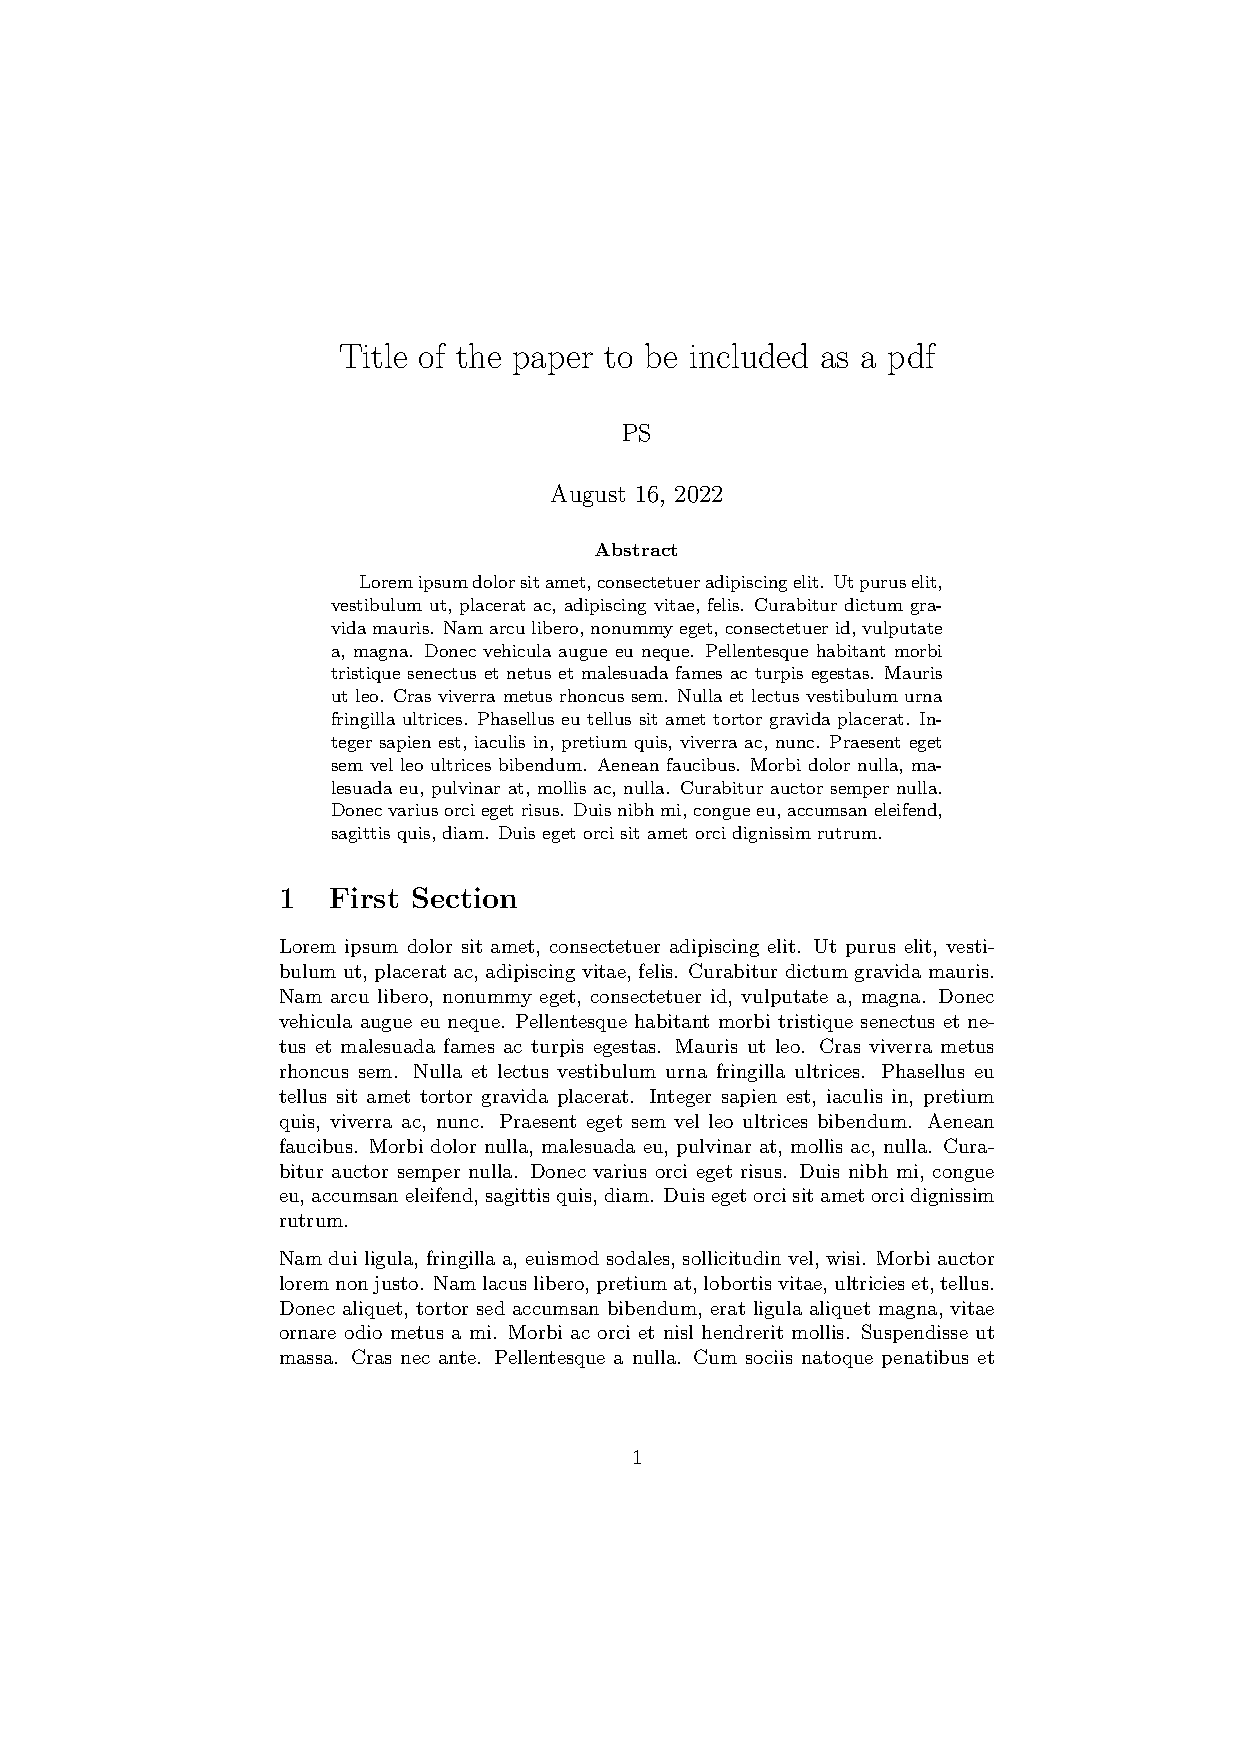
\includepdf[pages=1, noautoscale=false,scale=0.86] {./papersToInclude/paper2/paper2pdfInclude.pdf}

\includepdf[pages=2-21,pagecommand={\thispagestyle{standardThesisPdfInclude}},noautoscale=false,scale=0.86] {./papersToInclude/paper2/paper2pdfInclude.pdf} 



\pagestyle{standardThesis}
\fancyhead[LE]{\bfseries Paper III} 
\fancyhead[RO]{\bfseries \TitlePaperIII}

\setcounter{section}{0}
\setcounter{table}{0}
\setcounter{figure}{0}
\setcounter{equation}{0}
\setcounter{footnote}{0}

\chapter*{} %This is a dummy chapter to get the links/Bookmarks correct
\addcontentsline{toc}{chapter}{\texorpdfstring{Paper III \protect\tabto{1.5cm}--- %
\protect\parbox[t]{250pt}{\TitlePaperIII}}{Paper III}
}

\thispagestyle{empty}
\thumbWithColor[black]{Paper III}

\newpage
\thispagestyle{empty}
\vspace*{\fill}

%% **** IF THE PAPER IS PUBLISHED ****
%This paper has been published as: 
%
%\fullciteAllNames{SoderbackBlomvallSingull2021div}
%
%% **** IF ADDITIONAL INFORMATION ARE OF INTEREST ****
%\textbf{Open Access} This article is distributed under the terms of the Creative Commons Attribution 4.0 International License (\url{http://creativecommons.org/licenses/by/4.0/}), which permits unrestricted use, distribution, and reproduction in any medium, provided you give appropriate credit to the original author(s) and the source, provide a link to the Creative Commons license, and indicate if changes were made.

\begin{refsection}

%%%
% Users can, if they want, define newcommands and similar things in this space
%%%

\thispagestyle{empty}

\begin{center}
	{Title Paper 3}\\
	
	\vspace{0.20cm}
	
	\textbf{Author 1}\\
	Division of Author 1\\
	Department of Author 1\\
	
	\vspace{0.12cm}
	
	\textbf{Author 2}\\
	Division of Author 2\\
	Department of Author 2\\
	
	\vspace{0.12cm}
\end{center}

\textbf{Abstract: }\lipsum[1]

\textbf{Keywords: } Keyword ; Keyword; Keyword; Keyword; Keyword; Keyword
\clearpage

Paper three only use the reference \cite{CarrYu2012}

\lipsum[1-15]
\begin{figure}
Figure in paper 3
\caption{figure text in paper 3}
\end{figure}
\lipsum[1-15]

\printbibliography
\clearpage

\setcounter{section}{0}
\def\thesection{Appendix \Alph{section}}

\def\thesection{\Alph{section}}
\section{Section title Appendix}
\lipsum[1]

\subsection{under title}
\lipsum[2-3]

\subsection{under title again}
\lipsum[4-5]

\section{Here is another Section in the Appendix}
\lipsum[6-7]


\def\thesection{\arabic{section}} %Reset A change made in the Appendix

\end{refsection}


\pagestyle{standardThesis}
\fancyhead[LE]{\bfseries Paper IV} 
\fancyhead[RO]{\bfseries \TitlePaperIV}

\setcounter{section}{0}
\setcounter{table}{0}
\setcounter{figure}{0}
\setcounter{equation}{0}
\setcounter{footnote}{0}

\chapter*{} %This is a dummy chapter to get the links/Bookmarks correct
\addcontentsline{toc}{chapter}{\texorpdfstring{Paper IV \protect\tabto{1.5cm}--- %
\protect\parbox[t]{250pt}{\TitlePaperIV}}{Paper IV}
}

\thispagestyle{empty}
\thumbWithColor[black]{Paper IV}

\newpage
\thispagestyle{empty}
\vspace*{\fill}

%% **** IF THE PAPER IS PUBLISHED ****
%This paper has been published as: 
%
%\fullciteAllNames{SoderbackBlomvallSingull2021div}
%
%% **** IF ADDITIONAL INFORMATION ARE OF INTEREST ****
%\textbf{Open Access} This article is distributed under the terms of the Creative Commons Attribution 4.0 International License (\url{http://creativecommons.org/licenses/by/4.0/}), which permits unrestricted use, distribution, and reproduction in any medium, provided you give appropriate credit to the original author(s) and the source, provide a link to the Creative Commons license, and indicate if changes were made.

\begin{refsection}

%%%
% Users can, if they want, define newcommands and similar things in this space
%%%

\thispagestyle{empty}

\begin{center}
	{Title Paper 4}\\
	
	\vspace{0.20cm}
	
	\textbf{Author 1}\\
	Division of Author 1\\
	Department of Author 1\\
	
	\vspace{0.12cm}
	
	\textbf{Author 2}\\
	Division of Author 2\\
	Department of Author 2\\
	
	\vspace{0.12cm}
\end{center}

\textbf{Abstract: }\lipsum[1]

\textbf{Keywords: } Keyword ; Keyword; Keyword; Keyword; Keyword
\clearpage

Paper four do not use any references but use the \texttt{nocite} command to make all the reference appear in the list
\nocite{*}

\lipsum[31-40]
\begin{figure}
Figure in paper 4
\caption{figure text in paper 4}
\end{figure}
\lipsum[41-45]
\printbibliography
\clearpage

\setcounter{section}{0}
\def\thesection{Appendix \Alph{section}}

\def\thesection{\Alph{section}}
\section{Section title Appendix}
\lipsum[1]

\subsection{under title}
\lipsum[2-3]

\subsection{under title again}
\lipsum[4-5]

\section{Here is another Section in the Appendix}
\lipsum[6-7]


\def\thesection{\arabic{section}} %Reset A change made in the Appendix

\end{refsection}

\end{document}
